\documentclass[12pt]{article}
\parindent 0px

  	\usepackage[pdftex]{graphicx}
  	\graphicspath{{../pdf/}{../jpeg/}}
	\DeclareGraphicsExtensions{.pdf,.jpeg,.png}

	\usepackage[cmex10]{amsmath}
	\usepackage{mathabx}
	\usepackage{algorithmic}
	\usepackage{array}
	\usepackage{mdwmath}
	\usepackage{mdwtab}
	\usepackage{eqparbox}
	\usepackage{url}
        \usepackage{multirow}
        \usepackage{array}
	\hyphenation{op-tical net-works semi-conduc-tor}

\begin{document}

\title{
  \textbf{
    \textit{
      \LARGE Comparison of Models for SMS Spam Classification
      } 
    } 
  }

\author{
  Gyan Karthik Abhishek Sakibanda [110123230] \\
  sakiban@uwindsor.ca \\
  \and
  Karan Anandbhai Dhanwani [110122826] \\
  dhanwank@uwindsor.ca \\
  \and
  Shashank Kannan [110122650] \\
  kannan21@uwindsor.ca
}

\maketitle

\pagebreak

\section*{Abstract}
This study focuses on improving user experience, privacy, and security in SMS communication by automating the identification and filtering of unwanted and potentially harmful spam messages. The research employs Multinomial Naive Bayes for SMS spam classification and conducts a comparative analysis between a Custom implementation and a Built-in model from Scikit-Learn\cite{scikit-learn}. Additionally, the study explores the performance of these Machine Learning Models to evaluate their effectiveness in enhancing the accuracy and efficiency of spam detection in SMS communication. The findings contribute valuable insights into the development and optimization of spam filtering mechanisms, ultimately aiming to create a safer and more seamless user experience in mobile messaging.

\begin{quote}
\textbf{Keywords:} \textit{SMS communication, Spam messages, Multinomial Naive Bayes, Classification models, Spam detection.}
\end{quote}

% ===================
% # I. Introduction #
% ===================

\section{Introduction}
As mobile communication continues to play a pivotal role in daily interactions, the prevalence of unwanted and potentially harmful spam messages poses a significant challenge to user experience, privacy, and security\cite{sms-spam}. This research addresses this issue through the automatic identification and filtering of spam messages in SMS communication, with the overarching goal of enhancing the overall mobile messaging experience.\\

The primary focus of this study is the development and comparison of SMS spam classification models, employing the widely used Multinomial Naive Bayes algorithm. The utilization of this algorithm serves as a foundation for building robust models capable of distinguishing between legitimate and spam messages, thus contributing to the mitigation of potential threats to user privacy and security.\\

Two distinct approaches are explored in this research: a Custom implementation and the integration of a Built-in model from the renowned Scikit Learn library. By implementing a Custom model, the study aims to investigate the feasibility of tailoring the classification process to the specific nuances of SMS spam detection. Simultaneously, the incorporation of a Built-in model from Scikit Learn provides a benchmark for comparison, considering the expertise and optimization embedded in such established frameworks.\\

The core objective is to comprehensively compare the performance of these two approaches—Custom and Built-in models—assessing their accuracy, efficiency, and effectiveness in classifying SMS spam. Through a systematic evaluation, this research aims to provide insights into the strengths and weaknesses of each approach, offering valuable guidance for practitioners and researchers in the ongoing pursuit of enhancing SMS spam detection capabilities. The outcomes of this study have the potential to inform the development of more robust and adaptive models, contributing to a safer and more secure SMS communication environment.

% =============================================
% # II. Literature Survey #
% =============================================

\section{Literature Survey}

The purpose of this literature survey is to explore and compare various methodologies and algorithms that have been developed to tackle the issue of SMS spam.\\

Our survey spans a range of studies, each contributing unique insights into the classification of SMS as either spam (unsolicited and often malicious content) or ham (legitimate messages).

\begin{enumerate}
  \setlength\itemsep{1em}
  \item \textit{M. F. Benedetto, “Spam detection in SMS messages,” 2021}\cite{Benedetto_2021} \\\\
      The article details a sophisticated approach to combating SMS spam in the context of a large-scale social app, particularly in areas with limited internet connectivity. It discusses the development of a model and associated procedures to preserve user experience quality in the face of increasing spam activity. The model was developed in collaboration with XpertAI\cite{XpertAI_2021}. The article emphasizes the challenges of spam detection, differences between SMS and email spam, and the unique aspects of the project including data collection, extraction, parsing, and the modeling process.
      
    \pagebreak
    
  \item \textit{D. Dsilva, "Ham or Spam? SMS Text Classification with Machine Learning," 2018}\cite{Dsilva_2018} \\\\
    The article addresses the escalating issue of SMS spam, a consequence of the widespread use of mobile phones and the inadvertent sharing of personal contact information. It focuses on the application of the Naive Bayes machine learning model to classify SMS messages as spam or legitimate (ham). The article aims to explain why the Naive Bayes model is particularly effective for this task, highlighting its suitability for handling large volumes of text data and efficient processing. Additionally, it delves into the visualization of the dataset using word clouds, offering insights into common patterns and characteristics of spam messages. This approach provides a practical perspective on implementing and understanding SMS spam detection using machine learning and data visualization techniques.
\end{enumerate}

% ========================
% # III. Methodology #
% ========================

\section{Methodology}
The research uses the "SMS Spam Collection Dataset" available on Kaggle\cite{dataset_2016}, which comprises over 5,500 examples of labeled SMS messages categorized as ham (legitimate) or spam.\\

The methodology for the SMS spam classification study briefly encompasses the following key steps:

\subsection{Data Preprocessing}
Data preprocessing is a critical step, involving several sub-processes to convert raw SMS data into a clean, analyzable format. Initially, the data is cleansed to remove noise such as non-alphanumeric characters, unnecessary whitespace, and irrelevant symbols that could skew the analysis. Subsequently, tokenization breaks down text into individual words, and normalization standardizes these tokens to a base form, often involving converting all text to lowercase.\\

The frequency of each word is calculated to understand their distribution within the dataset. This process not only aids in identifying the most significant words for classification but also prepares the data for efficient processing by the subsequent machine learning models.

\subsection{Training and Test Set Creation}
The dataset is divided into training and test sets, a process crucial for both developing and objectively evaluating the model's performance. A typical split might allocate 80\% of the data for training and the remaining 20\% for testing. The division is performed in a stratified manner to ensure that the proportion of spam to ham messages is consistent across both sets, thereby preventing any bias that could result from an uneven distribution. This stratification helps to ensure that the model is trained and tested on data that represents the true nature of SMS communication, providing a reliable assessment of its classification ability.

\subsection{Model Development and Training}
The development and training stage of our methodology involves two primary tracks. First is the training of a custom-built Multinomial Naive Bayes model, designed to suit the specificities of SMS spam detection. This model is meticulously trained on the training set, allowing it to discern the intricate patterns that differentiate spam from legitimate messages.\\

The second track involves leveraging Built-in models provided by the Scikit-Learn library. These models come with the advantage of having been optimized based on a wide array of datasets and use cases, potentially offering a robust starting point for classification tasks.\\

Both the custom and built-in models undergo hyperparameter tuning— for the custom model, this is an exploratory process to determine optimal settings, while for the Built-in model, it's more about fine-tuning to align the model with the specifics of the SMS dataset. The training process is carefully monitored to prevent overfitting and to ensure that the models can generalize well to unseen data.\\

Alongside our custom Multinomial Naive Bayes model, we utilize a suite of Scikit-Learn models renowned for their text classification capabilities. Each model incorporates a TF-IDF (Term Frequency-Inverse Document Frequency)\cite{Simha_2021} transformer within the pipeline, which is crucial for normalizing the text data and highlighting the importance of each term. The pipeline is given in Figure \ref{pipeline}

\begin{figure}[!htbp]
    \centering
    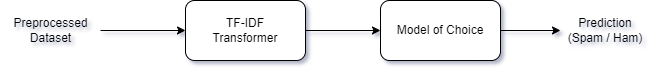
\includegraphics[scale=0.6]{Pipeline.png}
    \caption{Pipeline for training the Model}
    \label{pipeline}
\end{figure}    

The models we selected for comparison include:

\begin{enumerate}
    \item Logistic Regression
    \item Multinomial Naive Bayes Classification
    \item Random Forest Classifier
    \item Stochastic Gradient Descent (SGD)
\end{enumerate}

These models are trained using the TF-IDF vectorized text, allowing us to evaluate how different algorithms process and learn from the same transformed dataset.

\subsection{Model Evaluation}
Model evaluation is conducted with a keen focus on comparing the performance of the custom-built Multinomial Naive Bayes model against that of the built-in Scikit-Learn models. Accuracy is the first metric of comparison, providing a direct measure of how often the models correctly classify messages. To delve deeper into the models' performance, we generate confusion matrices for both, which pave the way to more detailed metrics such as precision, recall, and the F1 score. These metrics are particularly informative as they elucidate the balance between sensitivity to spam detection and the avoidance of misclassifying legitimate messages as spam.

% ============================
% # IV. Theoretical Approach #
% ============================

\section{Theoretical Approach}

The theoretical approach for the SMS spam classification research is rooted in the principles of supervised machine learning and natural language processing (NLP). We employ statistical algorithms to discern patterns in text data that can be used to classify messages as spam or ham. The theoretical foundation of each model used in the study is as follows:

\begin{enumerate}
\setlength\itemsep{1em}
    \item \textbf{Logistic Regression:} This model applies the logistic function to predict the probability that a given message belongs to a particular category. It's a binary classifier that assumes a linear relationship between the independent variables and the logarithm of the odds of the dependent variable.\cite{Molnar_2023} \\\\
    $P(y=1|x) = \frac{1}{1 + e^{-(\beta_0 + \beta_1 x_1 + \ldots + \beta_n x_n)}}$
    where,
    \begin{itemize}
    \setlength\itemsep{0.5em}
        \item $P(y=1|x)$ is the probability that message x is spam,
        \item $\beta_0$ is the intercept term, 
        \item $\beta_1$, ..., $\beta_n$ are the coefficients.
        \item $x_1$, ..., $x_n$ are the features.
    \end{itemize}
    
    \item \textbf{Multinomial Naive Bayes Classifier:} Based on Bayes' Theorem, this model assumes independence between predictors and applies to multinomially distributed data. It's particularly effective for document classification by calculating the conditional probability of each class given a word and then predicting the class with the highest probability.\cite{Chauhan_2022}
    \\\\
    $P(c|d) = P(c) \prod_{1}^{n} P(t_i|c)^{x_i}$
    where,
    \begin{itemize}
    \setlength\itemsep{0.5em}
        \item $P(c|d)$ is the posterior probability of class $c$ given document $d$.
        \item $P(c)$ is the prior probability of class $c$.
        \item $P(t_i|c)$ is the likelihood which is the probability of term $t_i$ occurring in a document of class $c$.
        \item $x_i$ is the frequency of term $t_i$ in document $d$. 
    \end{itemize}

    \item \textbf{Random Forest Classifier:} This ensemble method constructs multiple decision trees during training and outputs the class that is the mode of the classes predicted by individual trees. It introduces randomness into the model building to ensure that trees are de-correlated and reduces the variance of the final model.\cite{Saini_2022}
    \\\\
    $
    Y_{i} = \begin{cases} 
    1 & \text{if } \sum_{j} X_{ij} \cdot W_{j} + b_{i} \geq 0 \\
    0 & \text{otherwise} 
    \end{cases}
    $
    where,
    \begin{itemize}
    \setlength\itemsep{0.5em}
        \item $Y_i$ is the prediction at node $i$.
        \item $X_ij$ are the input features.
        \item $W_j$ are the learned weights.
        \item $b_i$ is the bias for node $i$.
    \end{itemize}
    
    The final classification is typically determined by a majority vote across all trees.

    \item \textbf{Stochastic Gradient Descent (SGD):} SGD is an iterative method for optimizing an objective function. In the context of machine learning, it's used to fine-tune the parameters of a model by minimizing the loss function, making it efficient for large datasets.\cite{Ruder_2020}
    \\\\
    $w_{k+1} = w_k - \eta_k \nabla L(w_k)$ where,
    \begin{itemize}
    \setlength\itemsep{0.5em}
        \item $w_k$ is the weight vector at iteration $k$.
        \item $\eta_k$ is the learning rate at iteration $k$.
        \item $\nabla L(w_k)$ is the gradient of the loss function with respect to the weights at iteration $k$.
    \end{itemize}
\end{enumerate}

% =====================
% # V. Experiment Results #
% =====================

\section{Experiment Results}

The primary objective of our experiment was to evaluate the effectiveness of various machine learning models in classifying SMS messages as either spam or ham (non-spam). This section presents the results obtained from the models: Logistic Regression, Multinomial Naive Bayes (Custom and Built-in), RandomForest Classifier, and Stochastic Gradient Descent. The performance of each model was assessed using confusion matrices and key performance metrics, including accuracy, precision, recall, and F1-score.

\subsection{Custom Implementation}
\subsubsection{Confusion Matrix}
The confusion matrix for the custom model is shown in Figure \ref{fig:custom-matrix}\\
    \begin{figure}[!htbp]
        \centering
        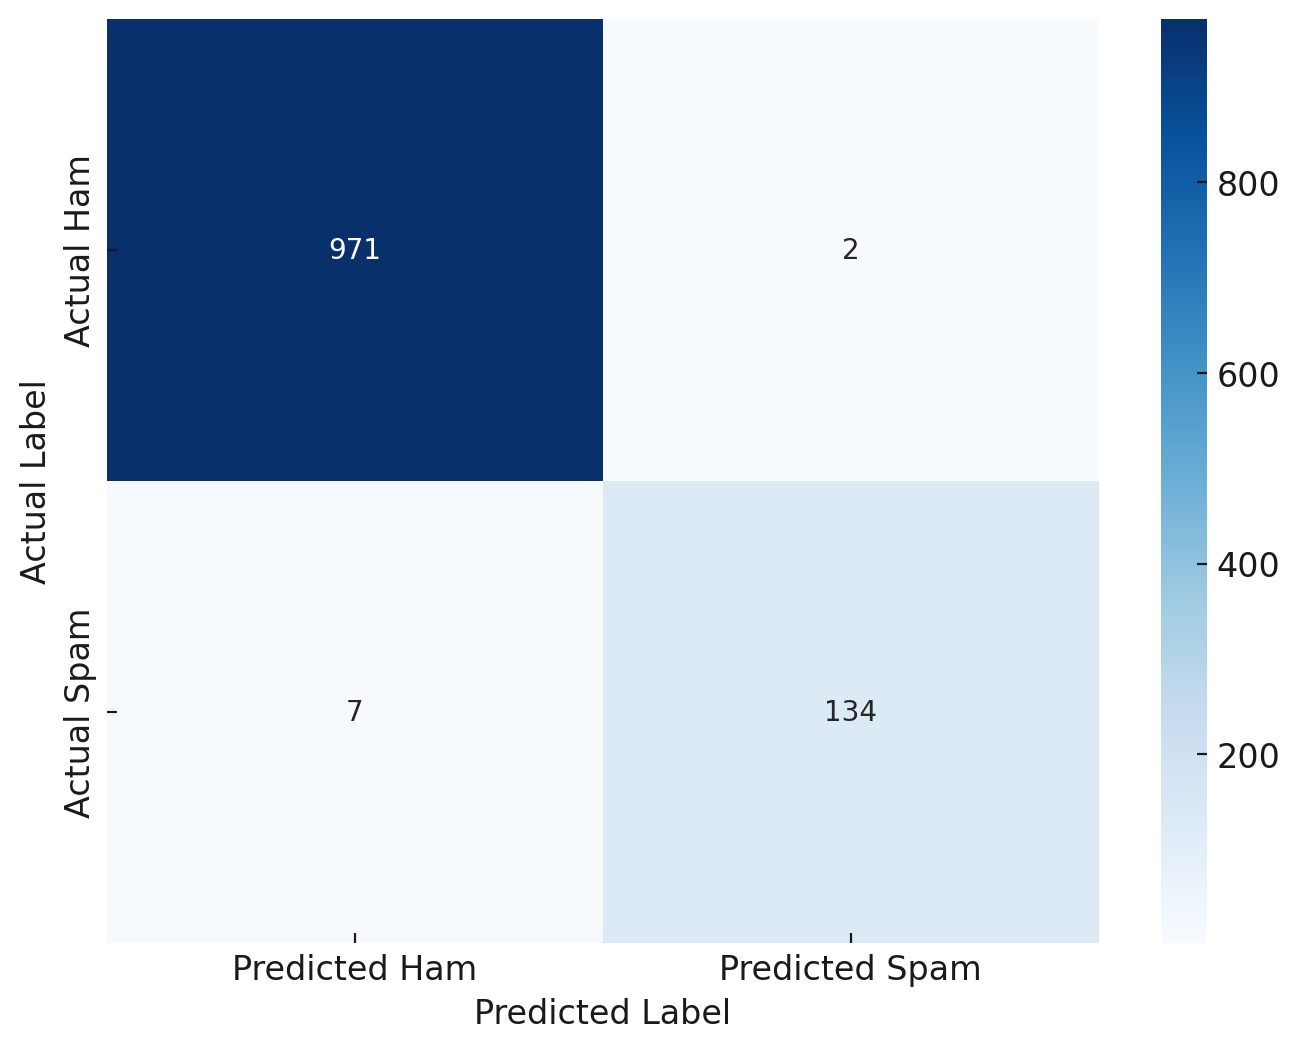
\includegraphics[width=0.77\linewidth]{matrix.png}
        \caption{Confusion Matrix for Custom Implemented Model}
        \label{fig:custom-matrix}
    \end{figure}

This matrix indicates a high number of true negatives, suggesting that the model is particularly effective at identifying ham messages. The low number of false positives is encouraging, as it implies minimal disruption to users from incorrectly classified ham messages. However, the presence of false negatives suggests some spam messages are still bypassing the filter.
\\
\subsubsection{Performance Metrics}
The custom implementation yielded the following performance metrics in Table \ref{tab:custom-performance_metrics}

\begin{table}[!htbp]
\centering
\begin{tabular}{|l|c|c|c|c|}
\hline
          & Precision & Recall & F1-score & Support \\ \hline
Ham       & 0.99      & 1.00   & 1.00     & 973     \\ \hline
Spam      & 0.99      & 0.95   & 0.97     & 141     \\ \hline
\multicolumn{4}{|l|}{Accuracy}             & 0.99    \\ \hline
\end{tabular}
\caption{Performance metrics for the custom SMS spam classification model}
\label{tab:custom-performance_metrics}
\end{table}

The SMS spam classification model showcases excellent proficiency, as indicated by these metrics. It achieves a precision of 0.99 and a full recall of 1.00 for ham messages, which signifies outstanding accuracy in correctly identifying non-spam messages with almost no errors. For spam messages, the model maintains an equally high precision of 0.99 and exhibits an impressive recall of 0.95, demonstrating its effectiveness in accurately detecting spam with only a small fraction of spam messages being misclassified. The F1-scores are notably high as well, with 1.00 for ham and 0.97 for spam, reflecting a superior balance between precision and recall for both categories. Overall, the model achieves an exceptional accuracy rate of 99\%, confirming its high efficiency in classifying spam and ham messages accurately. This performance underscores the model's reliability in both correctly filtering spam and safeguarding legitimate communications.

\subsection{Built-in Model}
\subsubsection{Confusion Matrix}
We could summarize the confusion matrices obtained from the four machine learning models are follows:

\begin{table}[!htbp]
\centering
\begin{tabular}{|l|c|c|}
\hline
           & Predicted Non-Spam & Predicted Spam \\ \hline
Actual Non-Spam & 948               & 1              \\ \hline
Actual Spam     & 39                & 127            \\ \hline
\end{tabular}
\caption{Confusion Matrix for Logistic Regression}
\label{tab:confusion_matrix_lr}
\end{table}

\begin{table}[!htbp]
\centering
\begin{tabular}{|l|c|c|}
\hline
           & Predicted Non-Spam & Predicted Spam \\ \hline
Actual Non-Spam & 949               & 0              \\ \hline
Actual Spam     & 33                & 133            \\ \hline
\end{tabular}
\caption{Confusion Matrix for Multinomial Naive Bayes}
\label{tab:confusion_matrix_nb}
\end{table}

\begin{table}[!htbp]
\centering
\begin{tabular}{|l|c|c|}
\hline
           & Predicted Non-Spam & Predicted Spam \\ \hline
Actual Non-Spam & 947               & 2              \\ \hline
Actual Spam     & 27                & 139            \\ \hline
\end{tabular}
\caption{Confusion Matrix for Random Forest Classifier}
\label{tab:confusion_matrix_rf}
\end{table}

\begin{table}[!htbp]
\centering
\begin{tabular}{|l|c|c|}
\hline
           & Predicted Non-Spam & Predicted Spam \\ \hline
Actual Non-Spam & 948               & 1              \\ \hline
Actual Spam     & 19                & 147            \\ \hline
\end{tabular}
\caption{Confusion Matrix for Stochastic Gradient Descent}
\label{tab:confusion_matrix_sg}
\end{table}

\begin{enumerate}
\setlength\itemsep{1em}
    \item \textbf{Logistic Regression:} (Table \ref{tab:confusion_matrix_lr})
    \begin{itemize}
    \setlength\itemsep{1em}
        \item Exhibited strong performance in correctly identifying non-spam messages with 948 true negatives (TN) and only 1 false positive (FP).
        \item However, it relatively underperformed in correctly classifying spam messages, with 39 false negatives (FN) and 127 true positives (TP).
    \end{itemize}

    \item \textbf{Multinomial Naive Bayes Classification:} (Table \ref{tab:confusion_matrix_nb})
    \begin{itemize}
    \setlength\itemsep{1em}
        \item Demonstrated excellent accuracy in identifying non-spam messages with 949 TN and no FP, outperforming other models in this aspect.
        \item Also showed improved performance in spam detection compared to Logistic Regression, with 33 FN and 133 TP.
    \end{itemize}

    \item \textbf{Random Forest Classifier:} (Table \ref{tab:confusion_matrix_rf})
    \begin{itemize}
    \setlength\itemsep{1em}
        \item Had a slightly lower performance than Multinomial Naive Bayes in detecting non-spam messages with 947 TN and 2 FP.
        \item However, it excelled in identifying spam messages, with the lowest number of FNs (27) and the highest number of TPs (139) among the models.
    \end{itemize}

    \item \textbf{Stochastic Gradient Descent:} (Table \ref{tab:confusion_matrix_sg})
    \begin{itemize}
    \setlength\itemsep{1em}
        \item Similar to Logistic Regression and Multinomial Naive Bayes in identifying non-spam messages with 948 TN and 1 FP.
        \item Remarkably, this model was the most effective in detecting spam with the highest TP rate (147) and the lowest FN rate (19) among the models.
    \end{itemize}
\end{enumerate}

\subsubsection{Performance Metrics} The performance metrics for the four models give the following insights:
\begin{itemize}
    \item The four machine learning models exhibit strong precision in spam detection, effectively minimizing false positives.
    
    \item Logistic Regression and Multinomial Naive Bayes show excellent precision but slightly lag in recall, indicating a tendency to miss some spam messages as shown in tables \ref{tab:performance_metrics_lr} and \ref{tab:performance_metrics_nb}.
    
    \item Random Forest Classifier as shown in table \ref{tab:performance_metrics_rf}, offers a more balanced performance with very good precision and better recall.
    
    \item Table \ref{tab:performance_metrics_sg} shows Stochastic Gradient Descent's performance metrics which emerged as the most effective, achieving the highest overall accuracy and a balanced mix of precision and recall, making it particularly proficient at correctly identifying both spam and non-spam messages.
\end{itemize}

\begin{table}[!htbp]
\centering
\begin{tabular}{|l|c|c|c|c|}
\hline
          & Precision & Recall & F1-Score & Support \\ \hline
Ham       & 0.96      & 1.00   & 0.98     & 949     \\ \hline
Spam      & 0.99      & 0.77   & 0.86     & 166     \\ \hline
\multicolumn{4}{|l|}{Accuracy}             & 0.96    \\ \hline
\end{tabular}
\caption{Performance Metrics for Logistic Regression}
\label{tab:performance_metrics_lr}
\end{table}

\begin{table}[!htbp]
\centering
\begin{tabular}{|l|c|c|c|c|}
\hline
          & Precision & Recall & F1-Score & Support \\ \hline
Ham       & 0.97      & 1.00   & 0.98     & 949     \\ \hline
Spam      & 1.00      & 0.80   & 0.89     & 166     \\ \hline
\multicolumn{4}{|l|}{Accuracy}             & 0.97    \\ \hline
\end{tabular}
\caption{Performance Metrics for Multinomial Naive Bayes Classification}
\label{tab:performance_metrics_nb}
\end{table}

\begin{table}[!htbp]
\centering
\begin{tabular}{|l|c|c|c|c|}
\hline
          & Precision & Recall & F1-Score & Support \\ \hline
Ham       & 0.97      & 1.00   & 0.98     & 949     \\ \hline
Spam      & 0.99      & 0.84   & 0.91     & 166     \\ \hline
\multicolumn{4}{|l|}{Accuracy}             & 0.97    \\ \hline
\end{tabular}
\caption{Performance Metrics for Random Forest Classifier}
\label{tab:performance_metrics_rf}
\end{table}

\begin{table}[!htbp]
\centering
\begin{tabular}{|l|c|c|c|c|}
\hline
          & Precision & Recall & F1-Score & Support \\ \hline
Ham       & 0.98      & 1.00   & 0.99     & 949     \\ \hline
Spam      & 0.99      & 0.89   & 0.94     & 166     \\ \hline
\multicolumn{4}{|l|}{Accuracy}             & 0.98    \\ \hline
\end{tabular}
\caption{Performance Metrics for Stochastic Gradient Descent}
\label{tab:performance_metrics_sg}
\end{table}

% =====================
% # V. Interpretations #
% =====================

\section{Interpretations}
Certain perceptions can be gained when comparing the confusion matrices and performance metrics of the custom implementation of the Naive Bayes Classifier and the four machine learning models used:
\begin{enumerate}
\setlength\itemsep{1em}
    \item \textbf{Balanced Performance of Custom Implementation:} The custom implementation excels in balancing both the identification of spam (high true positives) and the accuracy in classifying legitimate messages (low false positives), as reflected in its confusion matrix and performance metrics.

    \item \textbf{Comparative Strengths in Spam Detection:} Stochastic Gradient Descent and the custom implementation are particularly strong in detecting spam, with high true positive rates. Stochastic Gradient Descent slightly outperforms the custom model in recall, indicating better spam detection.

    \item \textbf{Precision and False Positives:}
    \begin{itemize}
        \item Multinomial Naive Bayes stands out for its perfect precision in spam detection, yet it has a slightly higher rate of missing spam messages (false negatives) compared to the custom implementation.
        \item Logistic Regression, while having a high precision, shows a tendency to miss more spam messages, as indicated by a higher false negative rate.
    \end{itemize}

    \item \textbf{Random Forest’s Balanced Approach:} Random Forest demonstrates a robust balance, closely mirroring the performance of the custom implementation with a slightly higher false positive rate but lower false negatives, indicating effective spam detection.

    \item \textbf{Overall Accuracy:} All models show high overall accuracy, with Stochastic Gradient Descent marginally leading, followed closely by the custom implementation.

    \item \textbf{F1-Score as an Indicator of Model Robustness:} The F1-score, which balances precision and recall, is notably high for the custom implementation and Stochastic Gradient Descent, underscoring their effectiveness in both aspects of classification.
\end{enumerate}

% =====================
% # VII. Conclusion #
% =====================

\section{Conclusion}
Our research on SMS spam classification reveals that both custom and built-in machine learning models from scikit-learn have unique strengths in spam detection. The custom implementation exhibited a strong balance in precision and recall, excelling in minimizing false negatives. Stochastic Gradient Descent stood out among built-in models, particularly in its ability to identify spam with high accuracy. Multinomial Naive Bayes and Logistic Regression models from scikit-learn demonstrated high precision but varied in recall, highlighting the trade-offs inherent in different modeling approaches. This study underscores the effectiveness of machine learning in spam detection and suggests a nuanced selection of models based on specific performance criteria.

% =====================
% # VII. Future Works #
% =====================

\section{Future Works}
We plan to extend our model comparison by including architectures from TensorFlow\cite{abadi2016tensorflow} and PyTorch\cite{NEURIPS2019_9015}, offering a deeper exploration into deep learning techniques. This expansion aims to uncover potential improvements in predictive performance. \\

Additionally, we aim to enhance the robustness and generalization of our models by diversifying the dataset beyond the SMS dataset used in the current study. Incorporating datasets with different characteristics, such as varied text sources, languages, or domains, will provide a more comprehensive evaluation of the models' adaptability and effectiveness across diverse contexts. \\

These future steps will contribute to a more nuanced understanding of model performance and strengthen the applicability of our findings across a broader spectrum of real-world scenarios.

\pagebreak

% ==============
% # REFERENCES #
% ==============

\bibliographystyle{IEEEtran}
\bibliography{biblio_traps_dynamics}

\end{document}
